\chapter{Results Discussion}

%\dots results discussion \dots 

%5.1
\section{Quantitative Results}
Thise section reports the results for {RQ$_1$} and {RQ$_2$}.

%Report precision/recall for different confidence thresholds
\textbf{RQ$_1$} \textit{How does our approach perform in detecting technical debt in unseen methods source code?} 

Table \ref{tbl:rq1} reports the precision, recall, accuracy and F1-score for twelve experiments on different dataset filtered by token count. The results using the smaller dataset, with tokens count less than 50 (dataset-50), shows the best precision (71\%), the second highest recall (62\%) and the best F1-score (66\%). The lowest F1-score (49\%) and lowest precision (42\%) are found with dataset-300. We notice that the second best precision (67\%) and the second highest F1-score comes with the largest dataset-600; this may lead to think that the size of the snippet influence the accuracy of the model only up to a point: in-fact we observe that the accuracy for larger dataset than 200 tokens remains roughly the same.

%https://www.tablesgenerator.com/#
\begin{table*}[h!]\centering
\ra{1.3}
\caption{Twelve experiments on different snippet sizes.\label{tbl:rq1}}
\begin{tabular}{@{}rrrrrr@{}}\toprule
\multicolumn{1}{r}{\#Tokens $< x$} &
  \multicolumn{1}{r}{\#Test samples} &
  \multicolumn{1}{r}{Prec.} &
  \multicolumn{1}{r}{Recall} &
  \multicolumn{1}{r}{Accuracy} &
  \multicolumn{1}{r}{F1-score} \\ 
\midrule
50  & 2826  & 71\% & 62\% & 64\% & 66\% \\ %run_id 6
100 & 8206  & 60\% & 62\% & 62\% & 61\% \\
150 & 12612 & 51\% & 63\% & 60\% & 56\% \\
200 & 15940 & 51\% & 60\% & 58\% & 55\% \\ %run_id 7
250 & 18518 & 47\% & 61\% & 58\% & 53\% \\
300 & 20346 & 42\% & 60\% & 57\% & 49\% \\
350 & 21712 & 53\% & 58\% & 57\% & 56\% \\
400 & 22782 & 60\% & 58\% & 58\% & 59\% \\ %run_id 40
450 & 23620 & 59\% & 57\% & 57\% & 58\% \\
500 & 24276 & 61\% & 57\% & 58\% & 59\% \\
550 & 24812 & 56\% & 58\% & 58\% & 57\% \\
600 & 25250 & 67\% & 56\% & 58\% & 61\% \\
\bottomrule
\end{tabular}
\end{table*}


\textbf{RQ$_2$} \textit{What is the correlation between the prediction confidence level and the accuracy of the model?}

We take two experiments from RQ$_1$ (dataset-50 and dataset-200) and analyze how the confidence level affects the quality metrics of the predictions. We observe that for the experiment in table \ref{tbl:rq2_token_50}, when filtering for a confidence level greater than 0.9 we reduce the coverage by 44\% gaining on precision from 71\% to 78\%; the excluded samples shows their effect also on the recall that goes from 62\% to 52\%. 
Table \ref{tbl:rq2_token_200} shows a different drop in coverage; with confidence greater than 0.9 the test set covered is about 2\%, the precision is high as 99\% and the recall drops to 10\%, both due to the (correct and incorrect) discarded predictions.
 
Figure \ref{fig:rq2_box_plot} presents, via box plots, the confidence level divided by class (i.e true positive, true negative, false positive and false negative) for both experiments. The plot shows a much greater confidence when using the smaller dataset: the median for the true positive dataset-50 is 0.97 and 0.56 for dataset-200.

\begin{table*}[h!]\centering
\ra{1.3}
\caption{Experiment `\#Tokens $< 50$' split for prediction confidence.\label{tbl:rq2_token_50}}

\begin{tabular}{@{}rrrrrr@{}}
\toprule
  \multicolumn{1}{r}{\#Confidence $> x$} &
  \multicolumn{1}{r}{\#Test samples} &
  \multicolumn{1}{r}{Test samples coverage} &
  \multicolumn{1}{r}{Prec.} &
  \multicolumn{1}{r}{Recall} &
  \multicolumn{1}{r}{F1-score} \\ 
\midrule
0   & 2826 & 100\% & 71\% & 62\% & 66\% \\
0.6 & 2592 & 92\%  & 72\% & 61\% & 66\% \\
0.7 & 2345 & 83\%  & 74\% & 59\% & 66\% \\
0.8 & 2027 & 72\%  & 76\% & 57\% & 65\% \\
0.9 & 1590 & 56\%  & 78\% & 52\% & 63\% \\
\bottomrule
\end{tabular}
\end{table*}

\begin{table*}[h!]\centering
\ra{1.3}
\caption{Experiment `\#Tokens $< 200$' split for prediction confidence.\label{tbl:rq2_token_200}}

\begin{tabular}{@{}rrrrrr@{}}
\toprule
  \multicolumn{1}{r}{\#Confidence $> x$} &
  \multicolumn{1}{r}{\#Test samples} &
  \multicolumn{1}{r}{Test samples coverage} &
  \multicolumn{1}{r}{Prec.} &
  \multicolumn{1}{r}{Recall} &
  \multicolumn{1}{r}{F1-score} \\ 
\midrule
0   & 15940 & 100\% & 51\% & 60\% & 55\% \\
0.6 & 4761  & 30\%  & 61\% & 34\% & 44\% \\
0.7 & 1616  & 10\%  & 79\% & 20\% & 32\% \\
0.8 & 757   & 5\%   & 92\% & 14\% & 25\% \\
0.9 & 349   & 2\%   & 99\% & 10\% & 18\% \\ 
\bottomrule
\end{tabular}
\end{table*}

%includere i box plot
\begin{figure}[h!]
 \centering
 \resizebox{\columnwidth}{!}{
  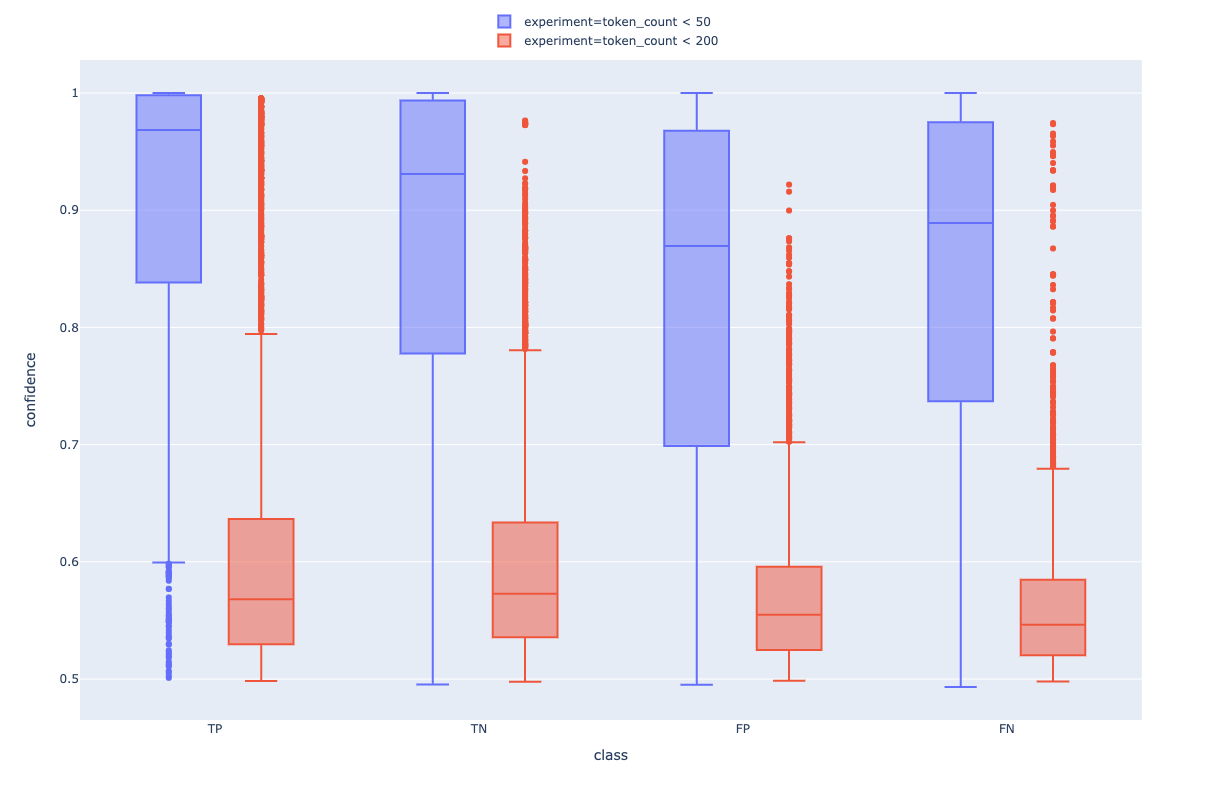
\includegraphics{images/box_plot.png}
 }
 \caption[Prediction confidence level split by class.]{Prediction confidence level split by class.}
    \label{fig:rq2_box_plot}
\end{figure}


%5.2 
\section{Qualitative Results}
%Discuss interesting cases in which your approach succeeds/fails
%, trying to explain what could make the model failing in those cases.

We discuss some qualitative examples where our model prediction succeed and where it fails. Then we explain why it was so.
We focus on high confidence predictions (correct and incorrect) using the following two scenarios, the same discussed in RQ$_2$:
\begin{itemize}
    \item Scenario-1: trained with a dataset composed only of those snippets with token\_count less than 50. The test dataset contains 1,413 sample pairs.
    %6,595 training sample pairs.
    \item Scenario-2: trained with a dataset composed only of those snippets with token\_count less than 200. The test dataset contains 7,970 sample pairs. This was the target of the hyperparameters tuning experiment.
    %37,195 training sample pairs.
\end{itemize}

All test session results are stored into a database with the information related to the prediction: a boolean value indicating if it was correct or incorrect, the confidence rating and some information on the attention vector weights. Each record contains these fields in pairs, one for the SATD and one for the fixed. It contains also the identifier link to trace back to the method source code and all related data.

The following paragraphs explain the findings for specific cases of both schenarios.

\textbf{Correct predictions, Scenario-1.} We queried Scenario-1 filtering for those samples that were correctly predicted with confidence greater than 0.99; the filter was applied to both elements of the pair at the same time, so both SATD/fixed were true positive with a high confidence rating.

Then, we manually went through a few of the 91 query hits, inspecting the source code of the SATD; we found the following interesting recurring cases:
\begin{itemize}
    \item Case-1 Empty exception block %id-125475
    \item Case-2 Magic constant %id-66085
    \item Case-3 Return null %id-57467
\end{itemize}

For each of these cases we extracted the weights of the attention vector and the related AST-paths, for both labels: SATD and fixed\footnote{The appendix section \ref{app:qualitative} contains the clean source code snippets of these three cases, the prediction confidence and the attention weights with the AST-paths}. These weights are sorted in descending order; looking at those values, we noticed that the first AST-path weight was roughly twice than the second. This means that the first AST-path was pivotal for the correct prediction. If the AST-path was decisive, it suggests it should be present in a meaningful way in the training set. After fixing the representation of the AST-path to the same stored in the database, we searched all the occurrences of the first particular path in this session training dataset samples. We also inspected the general distribution of weights and explained the most important AST-paths.


\begin{lstlisting}[caption={Case-1 SATD, verbatim source code}, label={lst:case_empty_exception},language=Java]

public boolean postfire() throws IllegalActionException {
    generateEvents(new ExecEvent(this, 2));
    try {
        Thread.sleep(100);
    } catch (InterruptedException e) {
        // FIXME
    }
    return super.postfire();
}

\end{lstlisting}

\begin{lstlisting}[caption={Case-1 fixed, verbatim source code}, label={lst:case1fixed},language=Java]
public boolean postfire() throws IllegalActionException {
    generateEvents(new ExecEvent(this, 2));
    try {
        Thread.sleep(100);
    } catch (InterruptedException e) {
        throw new InternalErrorException("Error with " + "sleeping thread in postfire");
    }
    return super.postfire();
}
\end{lstlisting}


\textbf{Case-1.} Using the first AST-path as a filter on the training dataset, we found three other cases labeled as SATD similar to this instance (see listing \ref{lst:case_empty_exception}). Then we inspected the fixed counterpart of this pair and found that the attention vector was giving roughly 45\% of the importance to the first three AST-paths; all of them has one end of the path in the \textit{throw new Exception} statement inside the \textit{catch} block (i.e. the fixed part of the snippet, see listing \ref{lst:case1fixed}). This could indicate that the model actually learned how to detect this particular technical debt with meaningful discriminating factors.


\textbf{Case-2.} `Magic constant' refers to the anti-pattern of using numbers directly in source code. In detail, Case-2 was found guilty for using the constant `302' to indicate the HTTP result code for \textit{StatusFound}. We inspected the first five AST-paths and searched for them throughout the training samples: we found 21 SATD with such paths. Four out of them were real `Magic constant' SATD, four were SATD related to a call to \textit{System.exit(0)} and the remaining were rich with numeric literals but not true `Magic constant' SATD. In other words, the positive element of this case was correctly classified not entirely for the right reasons.



\begin{lstlisting}[caption={Correctly detected SATD, verbatim Case-2}, label={lst:case_magic_constant},language=Java]

static void httpRedirect(final Exchange exchange, final String uri) {
    // FIXME: this constant should in HTTP package?
    httpResponse(exchange, 302);
    exchange.response.getHeaders().add(LocationHeader.NAME, uri);
}

\end{lstlisting}


\textbf{Case-3.} Returning null from a function is often associated with a bad smell. We went through the training samples with a common AST-path from Case-3 and we found three hits of SATD for a similar `return null'. We inspected other similar snippets to this case from Scenario-1 and found interesting different outcomes. We noticed methods containing a `return null' were correctly classified as negative (i.e. fixed): the code of such methods was using the arguments of the function before, eventually returning null; this changed the attention vector weights far from the `return null' statement. 


\begin{lstlisting}[caption={Case-3 SATD, verbatim source code}, label={lst:case3satd},language=Java]
public ItemStack constructTool(ItemStack rod, ItemStack... materials) {
    // FIXME: 1.11
    if (GemsConfig.TOOL_DISABLE_AXE)
        return null;
    return ToolHelper.constructTool(this, rod, materials);
}
\end{lstlisting}

\begin{lstlisting}[caption={Case-3 fixed, verbatim source code}, label={lst:case3fixed},language=Java]
public ItemStack constructTool(ItemStack rod, ItemStack... materials) {
    if (GemsConfig.TOOL_DISABLE_AXE)
        return ItemStack.EMPTY;
    return ToolHelper.constructTool(this, rod, materials);
}
\end{lstlisting}

\textbf{Wrong predictions, Scenario-1.}
The query yielded only one % id-43338
high confidence wrong prediction in contrast to the previous analysis where we had 91 correct high confidence predictions. Listing \ref{lst:scenario_1_wrong} contains both verbatim elements of the sample pair.


\begin{lstlisting}[caption={Scenario-1 wrong predictions, verbatim source code}, label={lst:scenario_1_wrong},language=Java]
//wrongly predicted as fixed
public String getClientID() {
    // fixme this will only work for 0-10 connections
    // In 0-8 there is an explicit ClientID property that is != Principal.
    return getPrincipal().getName();
}

//wrongly predicted as SATD
public String getClientID() {
    return getConnection().getClientId();
}
\end{lstlisting}

First we observe that the two snippets have the same AST structure: they share the same signature and return the value from two consecutive invocations. Thus, the AST-paths (excluding the value leaves) are identical. 
We analyzed the presence of such paths in the training samples. 
First we start with the actual SATD element (predicted as fixed), the easiest to explain; we traced the first two AST-paths and found that they recur most often in the fixed training samples: 15+44 (59) fixed occurrences versus 8+19 (27) SATD occurrences. 
Second, we explain the wrong prediction for the actual fixed element; this is more interesting because it has the same rough balance of before but leading to a different prediction. In-fact, the first two AST-paths have the following recurrence: 137+516 (653) fixed and 75+266 (341) SATD. Why did it predict with a SATD label and not a fixed? The answer lies in the number of samples that use both AST-paths at the same time: 75 SATD and 39 fixed. This ratio inversion was not present in the counterpart prediction above; the model took this into account as the dominant factor for the SATD prediction. 
%predicted:fixed actual:satd
%
% AST-path-1 50% string,1604992453,getprincipal
% satd  0 hit string,1604992453,getprincipal
% satd  1 hit string,1604992453,%
% satd  8 hit %,1604992453,%
% fixed 0 hit string,1604992453,getprincipal
% fixed 2 hit string,1604992453,%
% fixed 15 hit %,1604992453,%
%
% AST-path-2 22% METHOD_NAME,967193662,getprincipal
% satd  0 hit METHOD_NAME,967193662,getprincipal
% satd 19 hit METHOD_NAME,967193662,%
% satd 19 hit %,967193662,%
% fixed 0 hit METHOD_NAME,967193662,getprincipal
% fixed 44 hit METHOD_NAME,967193662,%
% fixed 44 hit %,967193662,%
%
% AST-path 1 & 2 1604992453&967193662
% satd 8 hit
% fixed 5 hit

%predicted:satd actual:fixed
% AST-path-1 32% string,270643758,getclientid
% satd  0 hit string,270643758,getclientid
% satd 21 hit string,270643758,
% satd 75 hit ,270643758,
% fixed 0 hit string,270643758,getclientid
% fixed 50 hit string,270643758,
% fixed 137 hit ,270643758,
%
% AST-path-2 23% METHOD_NAME,713917671,getclientid
% satd  0 hit METHOD_NAME,713917671,getclientid
% satd  266 hit METHOD_NAME,713917671,
% satd  266 hit 
% fixed 0 hit METHOD_NAME,713917671,getclientid
% fixed 516 hit METHOD_NAME,713917671,
% fixed 516 hit 
% 
% AST-path 1&2 270643758&713917671
% satd  75
% fixed 39
%
% AST-path-3 19% getconnection,1961396084,getclientid
% satd  0 hit getconnection,1961396084,getclientid 
% satd  0/0 hit *getconnection*,1961396084,*getclientid*
% satd  155 hit 1961396084
% fixed 0 hit getconnection,1961396084,getclientid 
% fixed 0/0 hit *getconnection*,1961396084,*getclientid*
% fixed 227 hit 1961396084
%
% AST-path-4 16% string,1604992453,getconnection
% satd  y hit 
% satd  y hit 
% satd  y hit 
% fixed y hit 
% fixed y hit 
% fixed y hit 

\textbf{Correct predictions, Scenario-2.}
 Querying Scenario-2 with confidence threshold set to 0.99 gave no hits; we lowered it to 0.87 and obtained ten sample pairs. This was probably due to Scenario-2 having a broader dataset that leads to a better generalization but brings in more noise. 
 Seven out of ten correct predictions were `return null' cases. We will explain one interesting case taken between the remaining three.


\begin{lstlisting}[caption={Scenario-2 correct predictions, verbatim source code}, label={lst:scenario_2_correct},language=Java]
public boolean contains(String s) {
    // FIXME
    return false;
}

public boolean contains(String s) {
    return containsHelper(s, root);
}
\end{lstlisting}

The model correctly labeled as SATD the method composed only of a `return false' statement. This is a consequence of not using the argument `s' of the method. On the other hand, the fixed counterpart was found to employ AST-paths involving the argument `s' in the evaluation of the return value.

\textbf{Wrong predictions, Scenario-2.}
We lowered the confidence ratio threshold to 0.7 and got four wrong prediction samples pair. This means that the model is less sure about the results probably due to the noisy dataset.
The actual fixed, wrongly predicted as SATD, are mainly `return null' that usually are actual SATD. In these cases, the fixes introduced the (normally) smelly code.